\documentclass[FIPLY_base.tex]{subfiles}

%\author{Gerald Irsiegler}
%\date{26. Februar 2016}

\begin{document}
\subsection{Statistik}

\subsubsection{Beschreibung}
Die Statistik gibt dem Benutzer eine Übersicht zu seinem Training in den letzen Tagen/Wochen/Monaten. 
\ \\
Es werden verschiedene Statistiken zur Verfügung gestellt, um dem Benutzer einen guten Überblick zu geben.

\begin{figure}[H]
	\begin{subfigure}[b]{0.3\textwidth}
	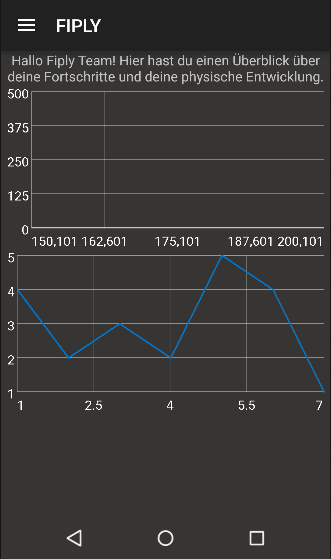
\includegraphics[scale=0.50]{img/Statistik}
	\end{subfigure}
	\hfil
	\caption{Die Statistik.}
\end{figure}

\subsubsection{Verfügbare Statistiken}
\paragraph{Geistige Verfassung}\ \\
Diese Statistik beschreibt wie es dem Benutzer nach jeder Trainingseinheit geht.
Er soll auf einer Skala von eins bis fünf seinen geistigen Zustand nach dem Training bewerten, wobei eine höhere Zahl eine bessere Laune beschreibt.
\paragraph{Gehobenes Gewicht}\ \\
Nach jeder Trainingseinheit wird angegeben mit wieviel Gewicht die jeweiligen Übungen durchgeführt worden sind.
Anhand dieser Statistik kann man den Muskelaufbau des Benutzers sehr gut verfolgen
\paragraph{Insgesamt gestemmtes Gewicht}\ \\
Hier wird festgehalten wieviel Gewicht der Benutzer insgesamt an einem Tag, einer Woche, einem Monat gestemmt hat.

\subsubsection{Implementierung}
\paragraph{Aufnahme und Speicherung der Werte}\ \\
Die aufzunehmenden Werte werden während bzw. nach der Trainingssession aufgenommen und danach in ihr jeweiliges Repository abgespeichert.
Die einzelnen Werte für die Statistik werden in einer SQLite Datenbank in ihren jeweiligen Repositories gespeichert.
\ \\
Dabei ist jeder Eintrag eine eigene Entität welche das Interface DataPointInterface implementiert.

\begin{lstlisting} [caption={Ein Datenpunkt für die Graphen.},label=DescriptiveLabel]
public class MoodTime implements DataPointInterface {
    private double _timestamp;
    private double _mood;

    public MoodTime(double timestamp, double mood) {
       _timestamp = timestamp;
       _mood = mood;
    }

    @Override
    public double getX() {
        return _timestamp;
    }

    @Override
    public double getY() {
        return _mood;
    }
}
\end{lstlisting}

\ \\

\paragraph{Darstellung}\ \\
Zur Darstellung der Statistiken wird GraphView verwendet. GraphView ist eine open-source Library für Android zur Erstellung von Diagrammen.
Verfügbar sind eine Vielzahl von Diagramm-Arten wie z.B.: Linien-, Kuchen- und Punktdiagrammen.


\end{document}
